\documentclass[11pt]{article}
\usepackage{amsmath,amssymb,booktabs,geometry,graphicx,hyperref,url}
\usepackage{array,float,placeins}
\hypersetup{hidelinks}
\geometry{margin=1in}
\graphicspath{{../output/figures/}{output/figures/}}
\setlength{\parskip}{0.45em}
\setlength{\parindent}{0pt}
\setlength{\emergencystretch}{2em}
\newcommand{\metricpair}[2]{\begin{tabular}[c]{@{}c@{}}#1\\[-0.15em]$\to$ #2\end{tabular}}

\title{PINN-Inspired Premium Regularization for Free-Boundary-Aware American Put Surrogates}
\author{SURF Project: Free-Boundary-Aware Risk Surfaces for American Options}
\date{July 3, 2026}

\begin{document}
\maketitle

\begin{abstract}
This report summarizes the Stage 21--23 PINN-inspired experiment campaign for the American-option risk-surface project. The campaign keeps Crank--Nicolson/projected successive over-relaxation (CN/PSOR) as the benchmark and label generator, and evaluates whether a PSOR-supervised positive-premium neural surrogate benefits from an auxiliary, masked Black--Scholes residual. Stage 21 established a small Option-B implementation but did not improve the matched supervised baseline. Stage 22 broadened the method search and found that terminal-premium variants improved price, boundary, and strict-\(\Delta\) metrics while worsening the masked PDE residual. Stage 23 retested terminal-scaled premium models with much stronger masked PDE regularization. Its best method, \path{terminal_pde_weight_5}, passed the capped candidate-success gate on all three seeds and improved price RMSE, masked residual mean absolute value, boundary RMSE, and strict-\(\Delta\) RMSE against the matched supervised neural baseline. This is a scoped surrogate result on the capped put campaign; it is not a claim that the neural model beats or replaces CN/PSOR.
\end{abstract}

\section{Executive Summary}

The campaign asked a narrow question: can a positive-premium neural surrogate trained from PSOR labels gain useful regularity from a masked PDE residual without weakening obstacle and boundary diagnostics? The answer from Stage 23 is yes within the tested capped put setting. The best Stage 23 method, \path{terminal_pde_weight_5}, reduced mean test price RMSE from \(0.06367\) to \(0.02223\), masked residual mean absolute value from \(0.05514\) to \(0.02806\), boundary RMSE from \(0.05974\) to \(0.01172\), and strict-\(\Delta\) RMSE from \(0.1025\) to \(0.09706\), relative to the matched supervised neural baseline.

The result should be framed carefully. The model remains a PSOR-supervised surrogate. CN/PSOR remains the numerical benchmark, the source of labels, and the source of the continuation-region mask. The evidence supports a future-extension claim that terminal scaling plus strong masked PDE regularization can beat a matched supervised neural baseline on this capped American put campaign.

\section{Claim Boundary and Scope}

The project's core benchmark is the CN/PSOR solver. The PINN-inspired experiments are deliberately downstream of that benchmark: PSOR labels define the supervised targets, PSOR diagnostics define the continuation mask, and PSOR remains the reference for price, premium, boundary, and Greek diagnostics.

The campaign is scoped to American puts from the Stage 05 surrogate dataset, using capped train/validation/test slices. The neural model predicts a nonnegative continuation premium \(\widehat C\), and normalized price is reconstructed as
\[
  \widehat u(x,\theta,r,q,\sigma,T)
  =
  \frac{\Phi}{K} + \widehat C(x,\theta,r,q,\sigma,T),
\]
where \(x=\log(S/K)\), \(\theta=\tau/T\), and \(\Phi/K\) is the normalized payoff obstacle. The positive-premium baseline uses a softplus output, so predicted price is obstacle-consistent by construction. The terminal-scaled model used in Stage 22 and Stage 23 multiplies the softplus premium by \(\theta\), enforcing zero continuation premium at expiry.

\section{Masked Residual Formulation}

The auxiliary residual is the log-space Black--Scholes continuation residual applied to the reconstructed normalized price:
\[
  \mathcal R(\widehat u)
  =
  \frac{1}{T}\widehat u_{\theta}
  - \frac{1}{2}\sigma^2 \widehat u_{xx}
  - \left(r-q-\frac{1}{2}\sigma^2\right)\widehat u_x
  + r\widehat u .
\]
The factor \(1/T\) on \(\widehat u_\theta\) is required because the dataset uses normalized maturity time \(\theta=\tau/T\), not raw time-to-maturity \(\tau\). The residual is used only as an auxiliary regularizer; it is not enforced globally and does not define an American-option solver.

The PDE mask is PSOR-derived:
\[
  \mathcal M_{\mathrm{PDE}}
  =
  \left\{
    i:
    u_i^{\mathrm{PSOR}}-\Phi_i/K>\epsilon,\,
    i\notin\mathrm{near\ boundary},\,
    i\notin\mathrm{near\ kink},\,
    \theta_i>\theta_{\min},\,
    i\in\mathrm{put\ scope}
  \right\}.
\]
In the campaign configuration, \(\epsilon=10^{-5}\) and \(\theta_{\min}=0.08\). This policy avoids exercise-region points, near-boundary samples, payoff-kink samples, near-maturity samples through the \(\theta\) threshold, and calls. The residual evaluation reports \path{psor_continuation_not_boundary_not_kink_not_maturity} as the mask source.

\section{Experiment Design}

\textbf{Stage 21.} The first run implemented the Option-B design: a small PSOR-supervised positive-premium MLP with a masked residual term. It used capped put samples, matched initialization against the supervised positive-premium baseline, and a small PDE weight. The run was diagnostic. Price RMSE and masked residual mean absolute value were slightly worse than the supervised baseline, so no improvement claim was supported.

\textbf{Stage 22.} The campaign then tested a broader method matrix across seeds 21, 22, and 23. Methods included fixed PDE-weight sweeps, warm-started PDE ramps, hard terminal premium scaling, residual-aware sampling, a strict-\(\Delta\) loss, and selected combinations. Success gates required price improvement, zero obstacle violation, masked residual non-regression, and boundary non-regression against the matched supervised baseline. The best Stage 22 method by the campaign ranking was \path{terminal_plus_ramp_plus_residual_sampling}. It improved price, boundary, and strict-\(\Delta\) metrics but worsened the masked residual enough to fail the candidate-success gate.

\textbf{Stage 23.} The final campaign diagnosed Stage 22 as a residual-strength issue. It retained the terminal-scaled architecture and retested stronger masked PDE regularization. The tested weights were \(\lambda_{\mathrm{PDE}}=2,5,10,25\), including selected residual-sampling variants. The best method was \path{terminal_pde_weight_5}. It passed candidate-success on all three seeds.

\section{Results}

Table~\ref{tab:full-method-coverage} lists the full method coverage before any best-method filtering. Stage 21 was a single matched diagnostic run, so it did not use the multi-seed candidate-success gate. Stage 22 and Stage 23 report candidate-success counts over three seeds.

\begin{table}[H]
\centering
\begingroup
\setlength{\tabcolsep}{3pt}
\scriptsize
\begin{tabular}{@{}l>{\raggedright\arraybackslash}p{0.46\linewidth}ccc@{}}
\toprule
Stage & Method & Gate count & Price RMSE & Masked residual \\
\midrule
21 & \path{supervised_positive_premium_mlp} & baseline & 0.09276 & 0.04594 \\
21 & \path{pinn_inspired_premium_mlp} & not gated & 0.09283 & 0.04619 \\
\addlinespace[0.2em]
22 & \path{supervised_baseline} & baseline & 0.09384 & 0.06806 \\
22 & \path{pde_weight_1e-6} & 0/3 & 0.09384 & 0.06806 \\
22 & \path{pde_weight_1e-5} & 0/3 & 0.09384 & 0.06806 \\
22 & \path{pde_weight_1e-4} & 0/3 & 0.09384 & 0.06806 \\
22 & \path{pde_weight_1e-3} & 0/3 & 0.09384 & 0.06802 \\
22 & \path{pde_ramp} & 0/3 & 0.09384 & 0.06806 \\
22 & \path{residual_sampling} & 0/3 & 0.09384 & 0.06805 \\
22 & \path{delta_loss} & 0/3 & 0.09384 & 0.06806 \\
22 & \path{terminal_premium} & 0/3 & 0.05111 & 0.14933 \\
22 & \path{terminal_plus_ramp} & 0/3 & 0.05110 & 0.14931 \\
22 & \path{terminal_plus_ramp_plus_residual_sampling} & 0/3 & 0.05110 & 0.14930 \\
\addlinespace[0.2em]
23 & \path{supervised_baseline} & baseline & 0.06367 & 0.05514 \\
23 & \path{terminal_pde_weight_2} & 3/3 & 0.02297 & 0.03559 \\
23 & \path{terminal_pde_weight_5} & 3/3 & 0.02223 & 0.02806 \\
23 & \path{terminal_pde_weight_10} & 3/3 & 0.02326 & 0.02512 \\
23 & \path{terminal_pde_weight_25} & 3/3 & 0.02782 & 0.02347 \\
23 & \path{terminal_pde_weight_10_residual_sampling} & 3/3 & 0.02500 & 0.02195 \\
23 & \path{terminal_pde_weight_25_residual_sampling} & 3/3 & 0.03133 & 0.02121 \\
\bottomrule
\end{tabular}
\endgroup
\caption{Full method coverage for the Stage 21--23 PINN-inspired campaign. Price RMSE and masked residual mean absolute value are test metrics; lower is better. Values are rounded from the generated coverage CSV, which is built from the committed Stage 21 metrics/residual CSVs and Stage 22--23 JSON summaries. Baseline rows are references rather than candidate methods.}
\label{tab:full-method-coverage}
\end{table}

\begin{table}[H]
\centering
\begingroup
\setlength{\tabcolsep}{3pt}
\scriptsize
\begin{tabular}{@{}l>{\raggedright\arraybackslash}p{0.28\linewidth}ccccc@{}}
\toprule
Stage & Best method & Successes & Price RMSE & Masked residual & Boundary RMSE & Strict-\(\Delta\) RMSE \\
\midrule
22 &
\path{terminal_plus_ramp_plus_residual_sampling} &
\(0/3\) &
\metricpair{0.09384}{0.05110} &
\metricpair{0.06806}{0.14930} &
\metricpair{0.08954}{0.05277} &
\metricpair{0.10950}{0.10206} \\
23 &
\path{terminal_pde_weight_5} &
\(3/3\) &
\metricpair{0.06367}{0.02223} &
\metricpair{0.05514}{0.02806} &
\metricpair{0.05974}{0.01172} &
\metricpair{0.10251}{0.09706} \\
\bottomrule
\end{tabular}
\endgroup
\caption{Best-method summary after the full method search in Table~\ref{tab:full-method-coverage}. Each metric is shown as matched supervised baseline \(\rightarrow\) candidate; lower is better. Values are rounded from the JSON/CSV artifacts in the Stage 22 and Stage 23 results directories.}
\label{tab:stage-comparison}
\end{table}

\begin{figure}[H]
\centering
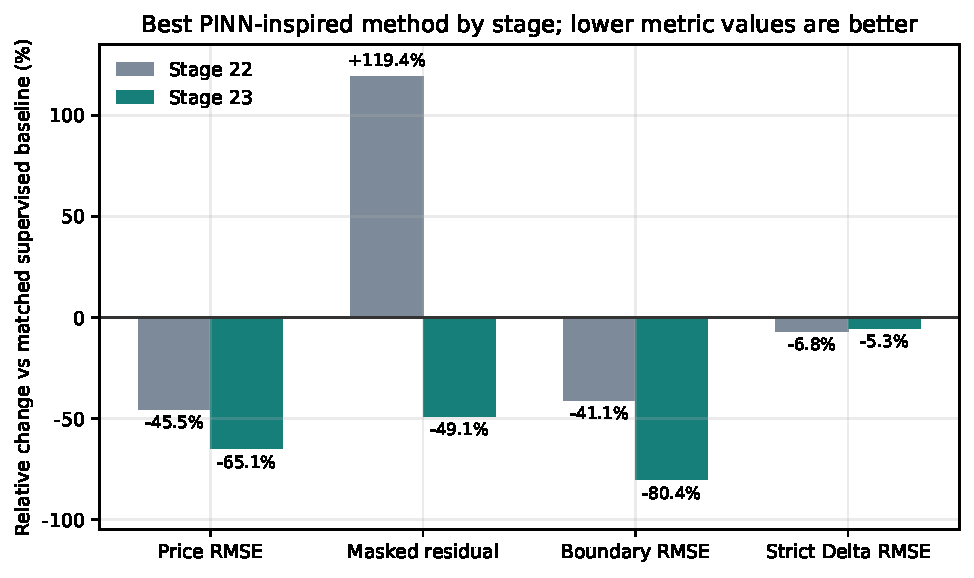
\includegraphics[width=0.88\linewidth]{pinn_stage22_stage23_relative_changes.pdf}
\caption{Relative metric changes for the best Stage 22 and Stage 23 methods after the full method search. Negative values indicate error reduction against the matched supervised baseline. Stage 22 improved three displayed supervised diagnostics but worsened the masked residual; Stage 23 improved all four displayed metrics.}
\label{fig:relative-changes}
\end{figure}

Tables~\ref{tab:full-method-coverage}--\ref{tab:stage-comparison} and Figure~\ref{fig:relative-changes} show the central contrast. Stage 22 identified terminal premium scaling as useful for supervised diagnostics but did not produce a residual-safe method. Stage 23 preserved the terminal scaling and increased the masked PDE regularization strength enough to improve the residual as well.

The Stage 23 method \path{terminal_pde_weight_5} improved mean price RMSE by about \(65.1\%\), masked residual mean absolute value by about \(49.1\%\), boundary RMSE by about \(80.4\%\), and strict-\(\Delta\) RMSE by about \(5.3\%\) against the matched supervised neural baseline. The largest gains are in price and boundary diagnostics. The Delta gain is modest but directionally favorable under the strict Greek mask.

\section{Interpretation}

The Stage 21 negative result was useful: simply adding a small masked residual to the positive-premium MLP did not improve the matched supervised baseline. Stage 22 then showed that terminal scaling solved part of the problem by making the premium architecture respect the expiry condition more directly, but it also exposed a tradeoff: price and boundary metrics could improve while the masked PDE residual deteriorated.

Stage 23 is the successful diagnostic retest. The stronger masked PDE penalty changed the tradeoff from ``better supervised diagnostics, worse residual'' to ``better supervised diagnostics and better residual.'' Because the mask is PSOR-derived and excludes boundary, kink, and maturity-sensitive points, the result is best understood as evidence that a terminal-scaled, PSOR-supervised surrogate can learn a smoother continuation-region premium on the capped put dataset.

This interpretation remains benchmark-first. The neural surrogate did not generate the exercise policy independently, did not solve the obstacle problem, and did not replace PSOR. It improved over a matched supervised neural baseline whose labels and masks still come from PSOR.

\section{Limitations}

The evidence is capped and put-only. The experiments use three seeds and capped training, validation, and test samples from the existing surrogate dataset, so broader regime coverage, larger training budgets, and uncapped evaluation would be needed before promoting the method beyond a future-extension surrogate result.

The residual is masked. It is evaluated only at PSOR continuation points away from the free boundary, payoff kink, and maturity threshold. This makes the diagnostic appropriate for the continuation PDE but does not validate the model at the exercise boundary or in the nonsmooth terminal region.

The strict-\(\Delta\) metric is a diagnostic, not a general Greek-engine claim. Stage 23 improves strict-\(\Delta\) RMSE modestly, but the project should continue to treat Greeks as separately audited quantities. Likewise, the boundary RMSE is a boundary-band diagnostic tied to the PSOR-generated dataset and should not be read as a standalone boundary solver.

\section{Conclusion}

The PINN-inspired campaign progressed from negative evidence in Stage 21, through a useful but residual-failing Stage 22 search, to a Stage 23 candidate that passed the capped success gate on all three seeds. The supported claim is precise: on the capped American put campaign, \path{terminal_pde_weight_5} beats the matched supervised positive-premium neural baseline on price, masked residual, boundary, and strict-\(\Delta\) diagnostics. CN/PSOR remains the benchmark and label generator.

\FloatBarrier

\section*{Reproducibility Artifacts}

\begin{itemize}\footnotesize
  \item Experiment plans and configuration:
  \path{docs/pinn_inspired_premium_experiment_plan.md};
  \path{configs/pinn_campaign.yaml};
  \path{configs/pinn_strong_terminal_campaign.yaml}.
  \item Stage scripts and model helpers:
  \path{experiments/21_pinn_inspired_premium.py};
  \path{experiments/22_pinn_campaign.py};
  \path{src/models/pinn_residual.py};
  \path{src/models/pinn_campaign.py}.
  \item Evidence summaries:
  \path{results/experiment_21_pinn_inspired_premium/pinn_summary.json};
  \path{results/experiment_22_pinn_campaign/pinn_campaign_summary.json};
  \path{results/experiment_23_pinn_strong_terminal/pinn_campaign_summary.json}.
  \item Figure and table generation:
  \path{scripts/plot_pinn_experiment_report.py};
  CSV outputs are under \path{results/figures/pinn_experiment_report/},
  and the comparison figure is under \path{output/figures/}.
\end{itemize}

\end{document}
